\documentclass[a4paper]{article}

\usepackage{préambule}

\title{Correction exercice 84 page 31}
\date{}


\begin{document}

\maketitle

On commence par dessiner à quoi ressemblerais notre solution. On dispose de pavés de longueur 60cm, de largeur 40cm et de hauteur 24cm. \vspace{1em}

\begin{greybox}
	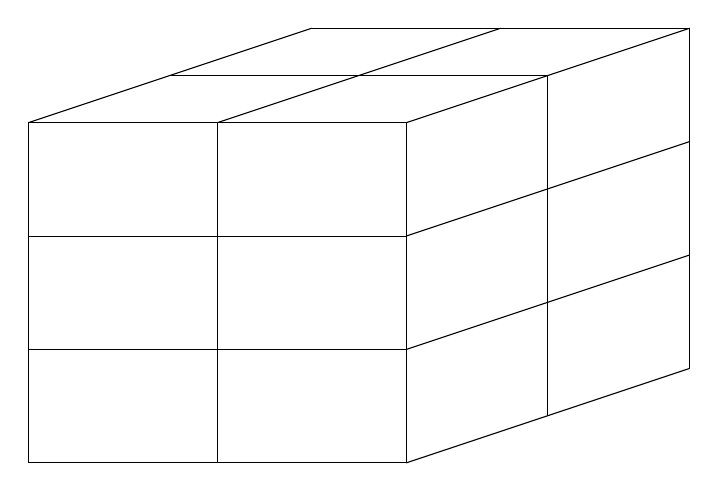
\begin{tikzpicture}[scale=0.6]
		% lignes verticales
		\draw (0,0) -- (0,7.2);
		\draw (4,0) -- (4,7.2);
		\draw (8,0) -- (8,7.2);
		\draw (11,1) -- (11,8.2);
		\draw (14,2) -- (14,9.2);
		% lignes horizontales
		\draw (0,0) -- (8,0);
		\draw (0,2.4) -- (8,2.4);
		\draw (0,4.8) -- (8,4.8);
		\draw (0,7.2) -- (8,7.2);
		\draw (3,8.2) -- (11,8.2);
		\draw (6,9.2) -- (14,9.2);
		% lignes diagonales
		\draw (0,7.2) -- (6,9.2);
		\draw (4,7.2) -- (10,9.2);
		\draw (8,7.2) -- (14,9.2);
		\draw (8,4.8) -- (14,6.8);
		\draw (8,2.4) -- (14,4.4);
		\draw (8,0) -- (14,2);
	\end{tikzpicture}

	Sur la figure ci-dessus, on a empilé 3 pavés en hauteur, 2 en longueur et 2 en largeur. Les dimensions de la figure obtenue sont 120cm de longueur, 80cm de largeur et 72cm de hauteur : ce n'est donc pas un cube.
\end{greybox}

On voit que la solution recherchée (la longueur du côté du cube) est nécéssairement un \textit{multiple} de 60, 40 et 24. De plus, on cherche le \textit{plus petit} tel multiple. On va donc utiliser le \textbf{PPCM} :

\begin{itemize}
	\item Décomposons d'abord 60, 40 et 24 en nombres premiers :

	      \begin{tabular}{c|c}
		      60 & 2 \\
		      30 & 2 \\
		      15 & 3 \\
		      5  & 5 \\
		      1  &
	      \end{tabular} \hspace{2em}
	      \begin{tabular}{c|c}
		      40 & 2 \\
		      20 & 2 \\
		      10 & 2 \\
		      5  & 5 \\
		      1  &
	      \end{tabular} \hspace{2em}
	      \begin{tabular}{c|c}
		      24 & 2 \\
		      12 & 2 \\
		      6  & 2 \\
		      3  & 3 \\
		      1  &
	      \end{tabular}

	      Donc $60 = 2×2×3×5$, $40 = 2×2×2×5$ et $24 = 2×2×2×3$.
	\item On calcule le PPCM de 60 et 40 :
	      $$ 60 = \cancel{2}×\cancel{2}×3×\cancel{5} $$
	      $$ 40 = \cancel{2}×\cancel{2}×2×\cancel{5} $$
	      $$ \text{de côté : } 2, 2, 5 $$

	      Donc le PPCM de 60 et 40 est $3×2×2×2×5 = 120$.
	\item On calcule le PPCM de 120 et 24 :
	      $$ 120 = \cancel{2}×\cancel{2}×\cancel{2}×3×\cancel{5} $$
	      $$ 24 = \cancel{2}×\cancel{2}×\cancel{2}×\cancel{3} $$
	      $$ \text{de côté : } 2, 2, 2, 5 $$

	      Donc le PPCM de 120 et 24 est $3×2×2×2×5 = 120$.
\end{itemize}

Ainsi le plus petit cube possible fait 120cm de côté.

\end{document}